\documentclass[12pt]{beamer}

\mode<presentation>{\usetheme{Warsaw}\setbeamercovered{transparent=5}}
\setbeamertemplate{footline}[frame number]
\usepackage[english]{babel}
\usepackage{times}
\usepackage{url}
\usepackage{graphicx}
\usepackage{listings}
\lstloadlanguages{Python}
\lstset{language=Python}
\lstset{%
	basicstyle=\ttfamily\bfseries,
	keywordstyle=\color{blue}, emph={self}, emphstyle={\color{blue}},
	identifierstyle=,
	commentstyle=\color{gray},
	stringstyle=\color{green!50!black},
	showstringspaces=false,
	emph={[2]__init__,__str__,hill_climb,simulated_annealing,DealerAgent,take_action}, emphstyle={[2]\color{purple}},
}
\newcommand{\key}[1]{{\color{blue}#1}}
\newcommand{\defn}[1]{{\color{purple}#1}}
\newcommand{\str}[1]{{\color{green!50!black}#1}}

\title{Informed Search and Exploration}
\subtitle{Introduction to Artificial Intelligence}
\author{Steven Bethard}
\institute{
  Department of Computer Science\\
  University of Colorado
}
\date{CSCI 3202}

\AtBeginSection[]{
  \begin{frame}<beamer>{Outline}
  	\footnotesize
    \tableofcontents[currentsection]
  \end{frame}
}

\begin{document}

\begin{frame}
  \titlepage
\end{frame}

\begin{frame}{Outline}
	\footnotesize
  \tableofcontents
\end{frame}

\section{Heuristic Search}
\begin{frame}{All States are not Equal}
	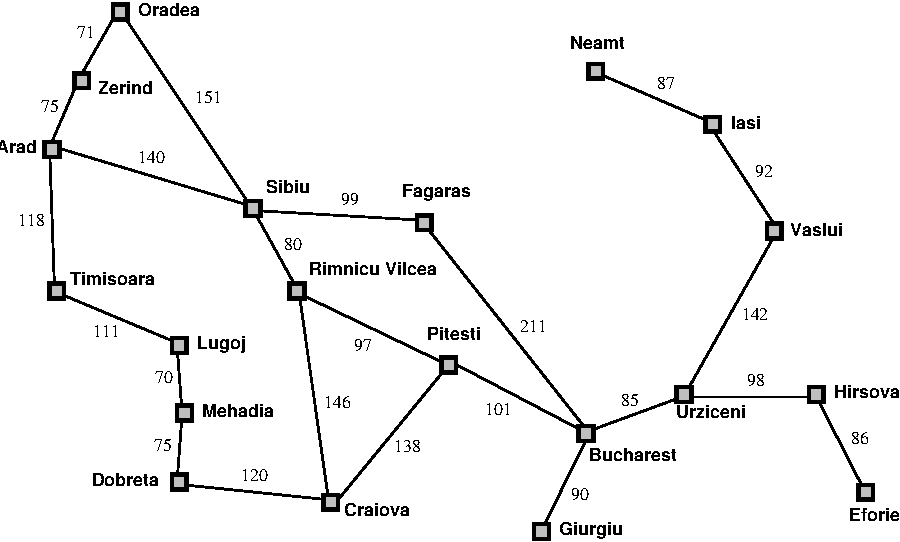
\includegraphics[width=4in]{romania-distances.pdf}
\end{frame}

\subsection{Best-First Search}
\begin{frame}{Best-First (Greedy) Search}
	\begin{center}
		\only<1>{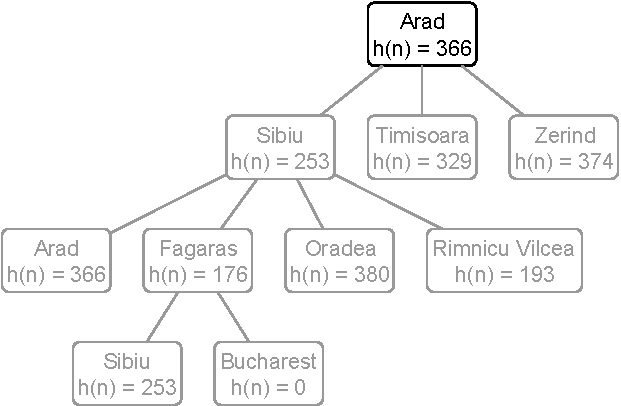
\includegraphics[height=2in]{greedy-1.pdf}}%
		\only<2>{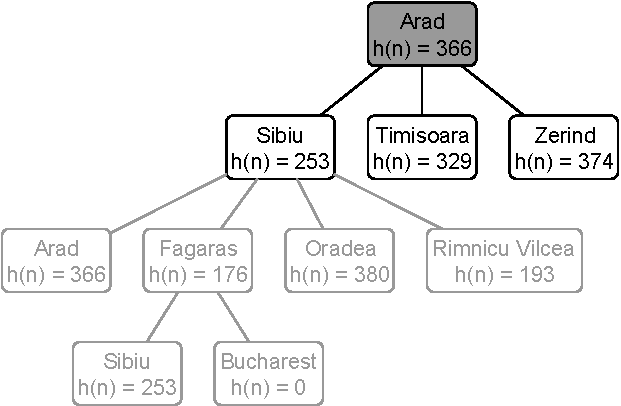
\includegraphics[height=2in]{greedy-2.pdf}}%
		\only<3>{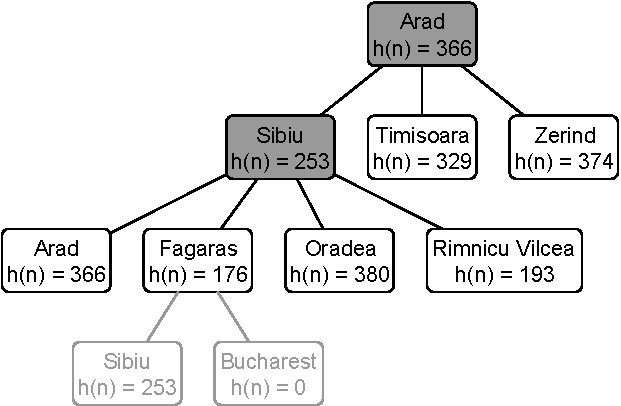
\includegraphics[height=2in]{greedy-3.pdf}}%
		\only<4>{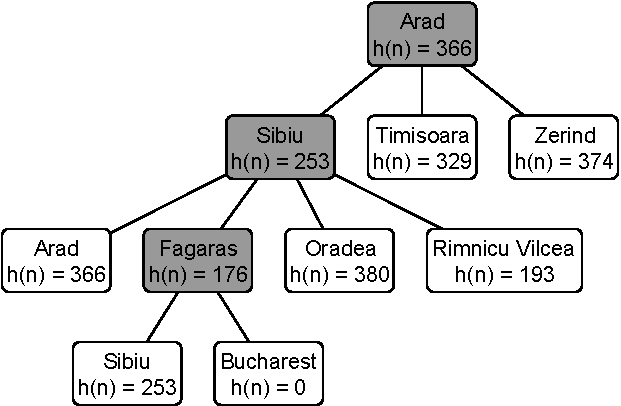
\includegraphics[height=2in]{greedy-4.pdf}}%
		\only<5>{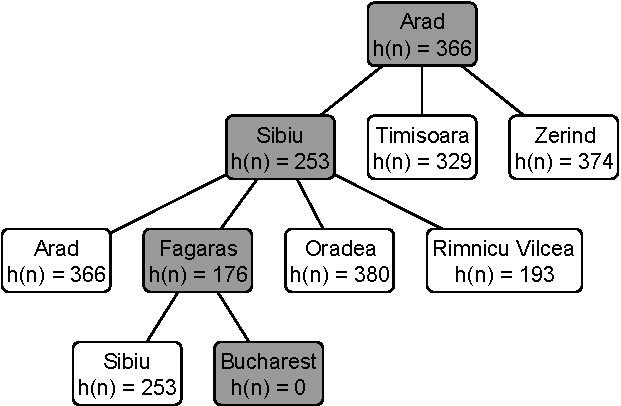
\includegraphics[height=2in]{greedy-5.pdf}}%
	\end{center}
\end{frame}
\begin{frame}{Best-First (Greedy) Properties}
	\footnotesize
	\begin{block}{Strategy?}
		 \uncover<2->{Priority Queue, $f(n) = h(n)$}
	\end{block}
	\begin{block}{Complete?}
		\uncover<3->{Yes, if finite number of states and no cyclic paths}
	\end{block}
	\begin{block}{Optimal?}
		\uncover<4->{No}
	\end{block}
	\begin{block}{Worst Case Time Complexity?}
		\uncover<5->{$O(b^m)$, but better with good heuristic}
	\end{block}
	\begin{block}{Worst Case Space Complexity?}
		\uncover<6->{$O(b^m)$}
	\end{block}
\end{frame}

\subsection{A* Search}
\begin{frame}{A* Search}
	\begin{center}
		\only<1>{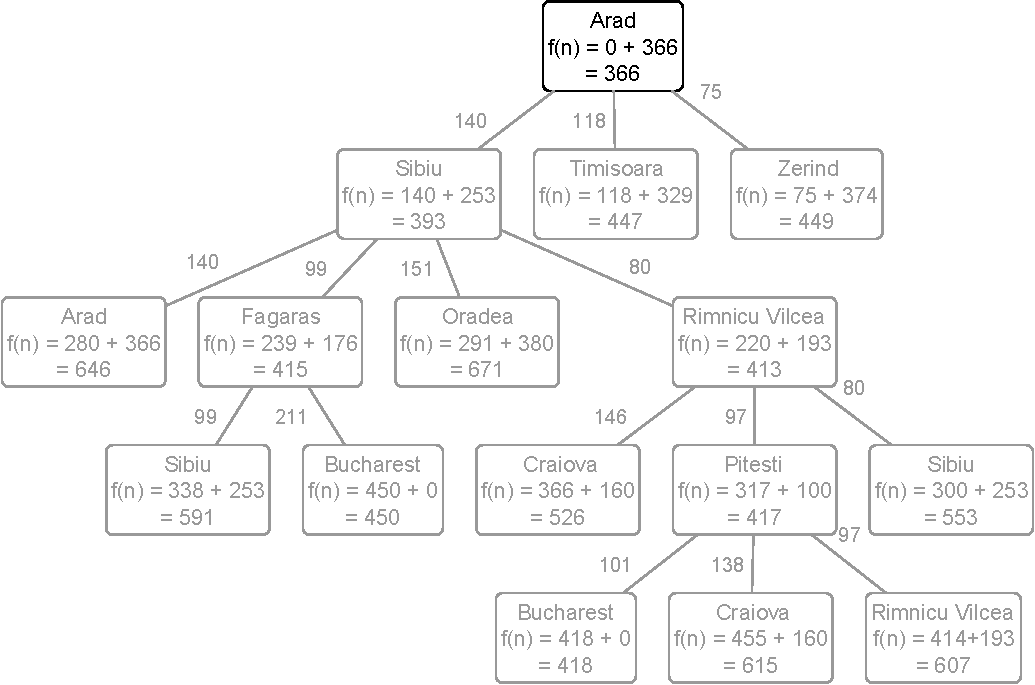
\includegraphics[height=2in]{a-star-1.pdf}}%
		\only<2>{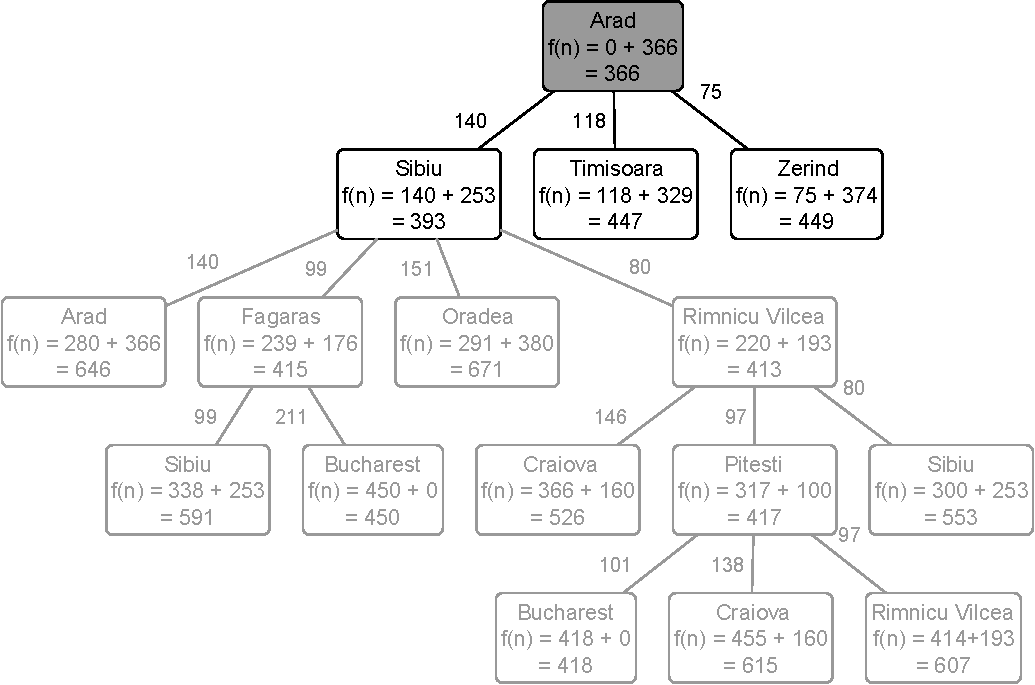
\includegraphics[height=2in]{a-star-2.pdf}}%
		\only<3>{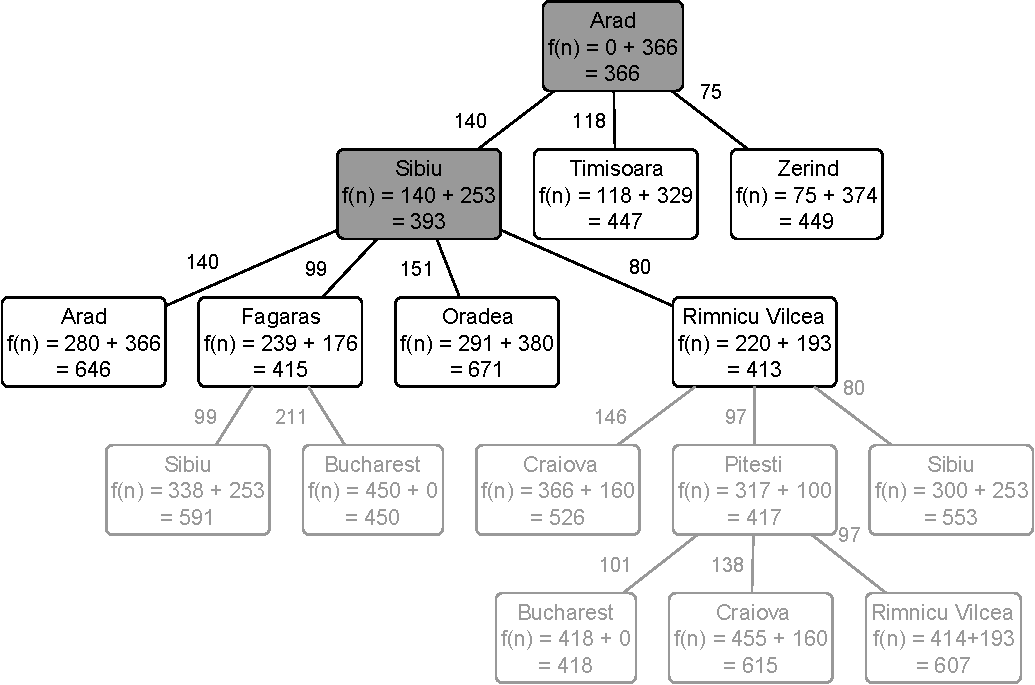
\includegraphics[height=2in]{a-star-3.pdf}}%
		\only<4>{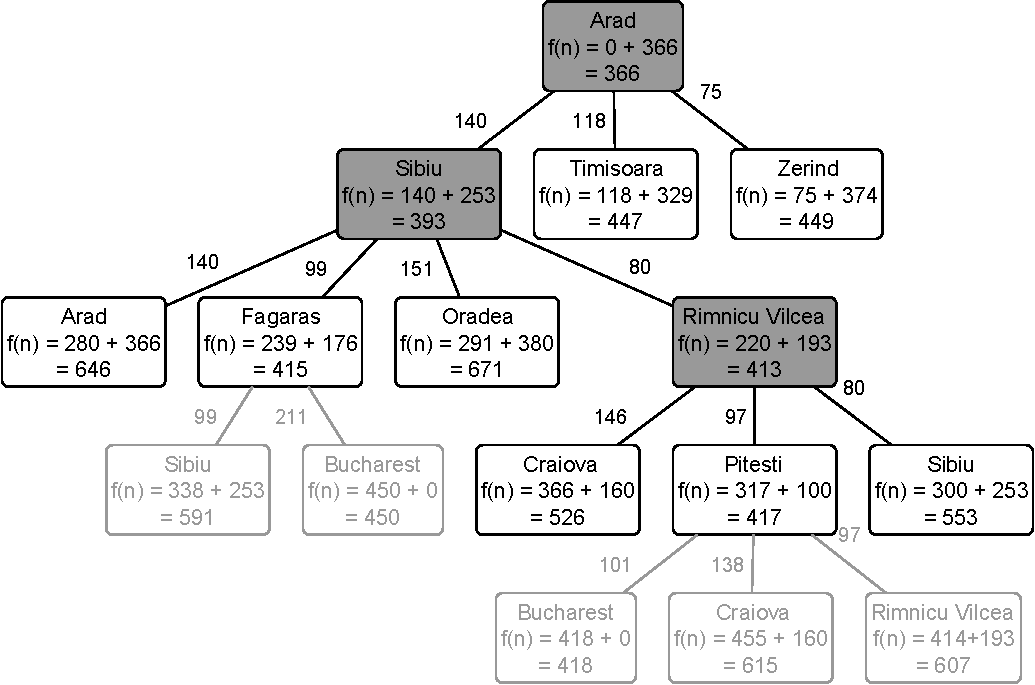
\includegraphics[height=2in]{a-star-4.pdf}}%
		\only<5>{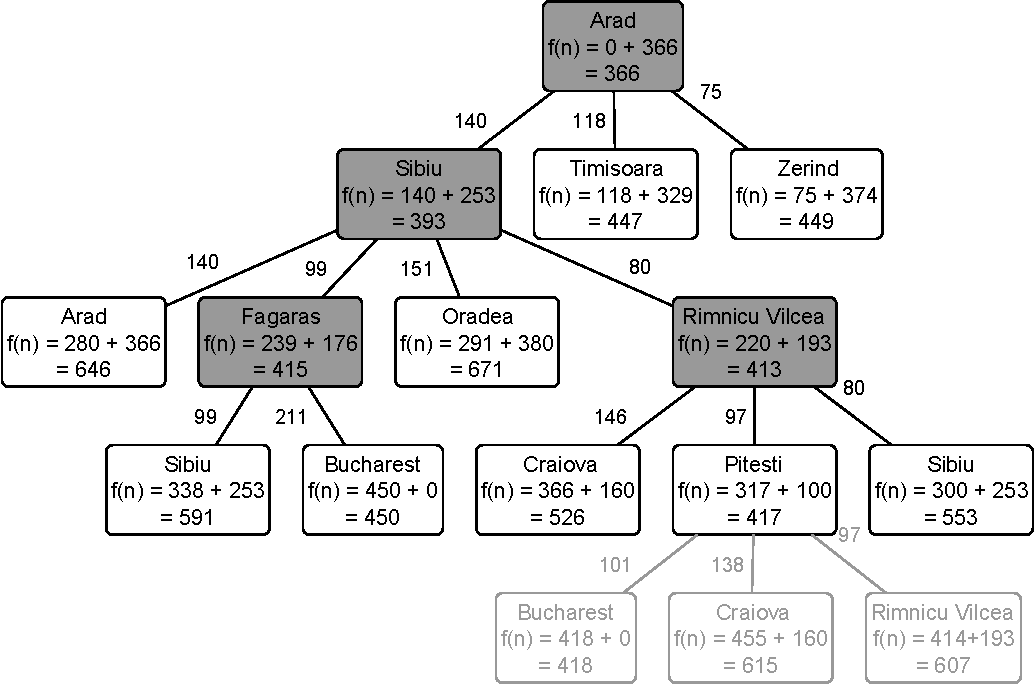
\includegraphics[height=2in]{a-star-5.pdf}}%
		\only<6>{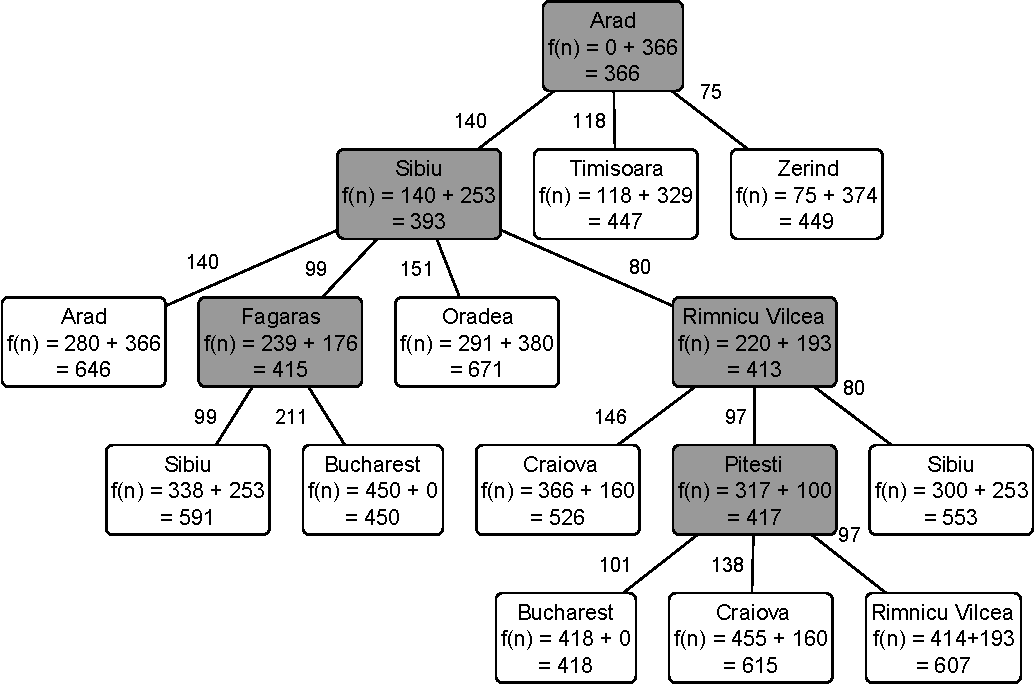
\includegraphics[height=2in]{a-star-6.pdf}}%
		\only<7>{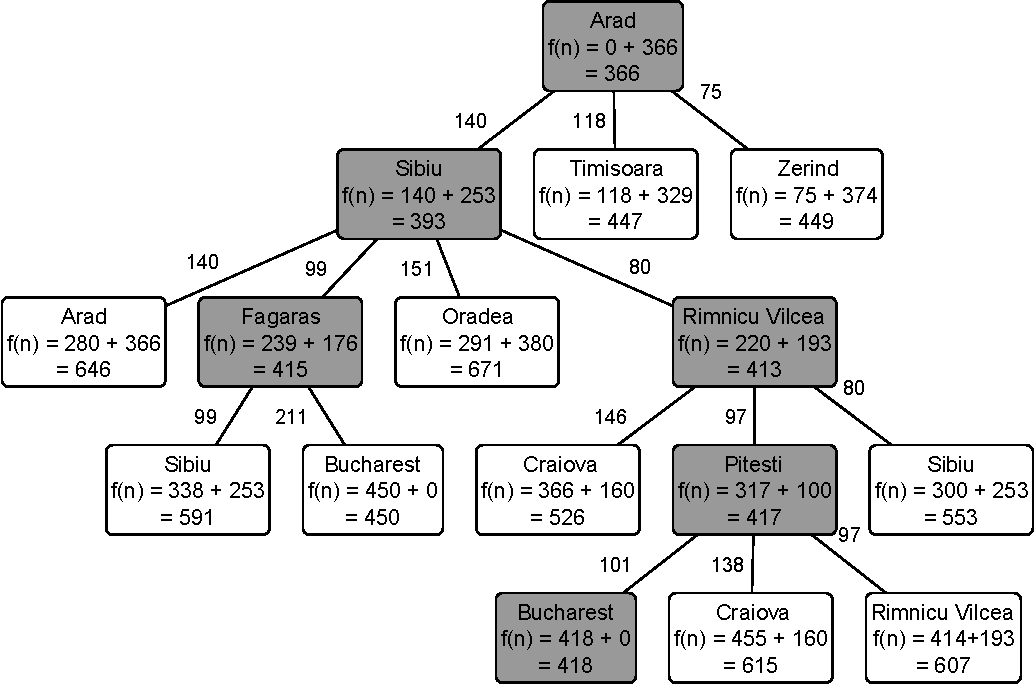
\includegraphics[height=2in]{a-star-7.pdf}}%
	\end{center}
\end{frame}
\begin{frame}{A* Properties}
	\footnotesize
	\begin{block}{Strategy?}
		 \uncover<2->{Priority Queue, $f(n) = g(n) + h(n)$}
	\end{block}
	\begin{block}{Complete?}
		\uncover<3->{Yes, if there are finite nodes with $f(n) < C^{*}$}
	\end{block}
	\begin{block}{Optimal?}
		\uncover<4->{Yes, if $h$ is consistent}
	\end{block}
	\begin{block}{Worst Case Time Complexity?}
		\uncover<5->{All nodes with $f(n) < C^{*}$, exponential in \texttt{len(path)}}
	\end{block}
	\begin{block}{Worst Case Space Complexity?}
		\uncover<6->{All nodes with $f(n) < C^{*}$}
	\end{block}
\end{frame}

\subsection{A* Optimality}
\begin{frame}{Proof that A* is Optimal}
	\begin{columns}[T]
		\begin{column}{1.75in}
			Suppose some suboptimal goal $G_2$ has been generated and is in the queue. Let $n$ be an unexpanded node on a shortest path to an optimal goal $G_1$.
		\end{column}
		\begin{column}{2.25in}
			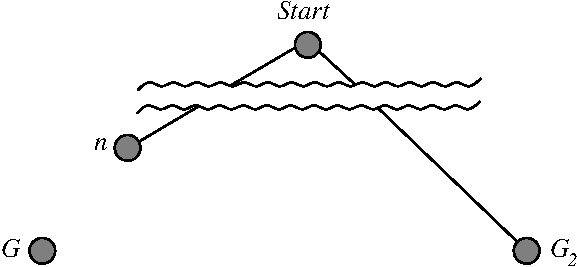
\includegraphics[width=2.25in]{a-star-proof.pdf}
		\end{column}
	\end{columns}
	\bigskip
	\[
	\begin{array}{llll}
	\uncover<2->{f(G_2)} & \uncover<2->{=  }  & \uncover<2->{g(G_2)} & \uncover<2->{\mbox{since $h(G_2) = 0$}} \\
	\uncover<3->{      } & \uncover<3->{>  }  & \uncover<3->{g(G_1)} & \uncover<3->{\mbox{since $G_2$ is suboptimal}} \\
	\uncover<4->{      } & \uncover<4->{\geq} & \uncover<4->{f(n)  } & \uncover<4->{\mbox{since $h$ is consistent}}
	\end{array}
	\]
	\bigskip
	\uncover<5->{Since $f(G_2) > f(n)$, A* will never select $G_2$ for expansion.}
\end{frame}
\begin{frame}{A* Contours}
	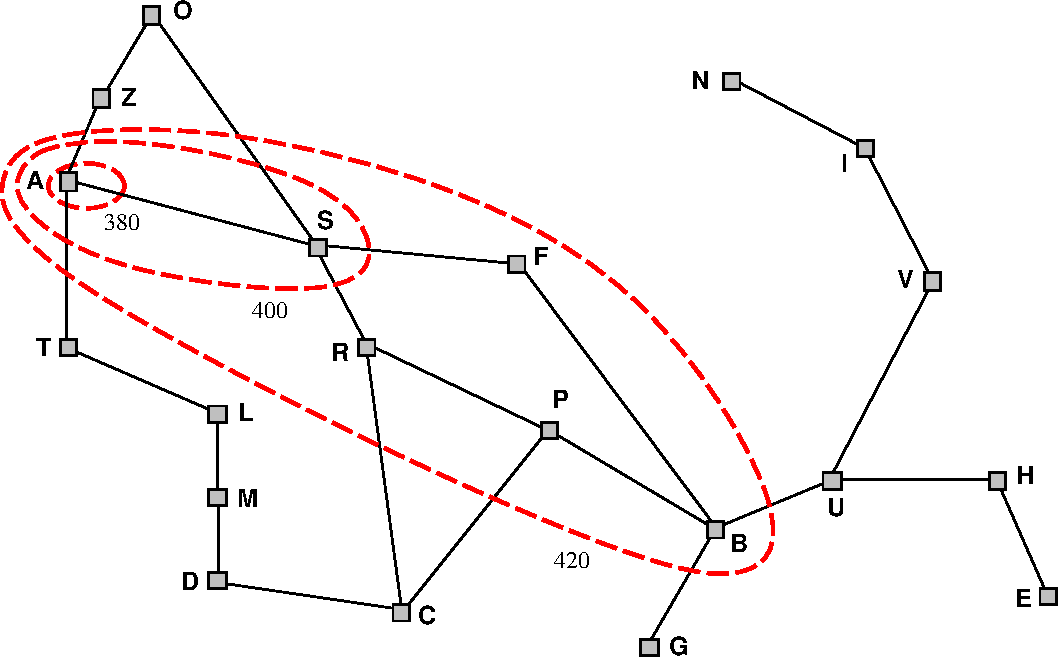
\includegraphics[width=4in]{a-star-contours.pdf}
\end{frame}

\section{Heuristic Functions}

\subsection{Heuristic Quality}
\begin{frame}{8-Puzzle Heuristics}
	\begin{center}
		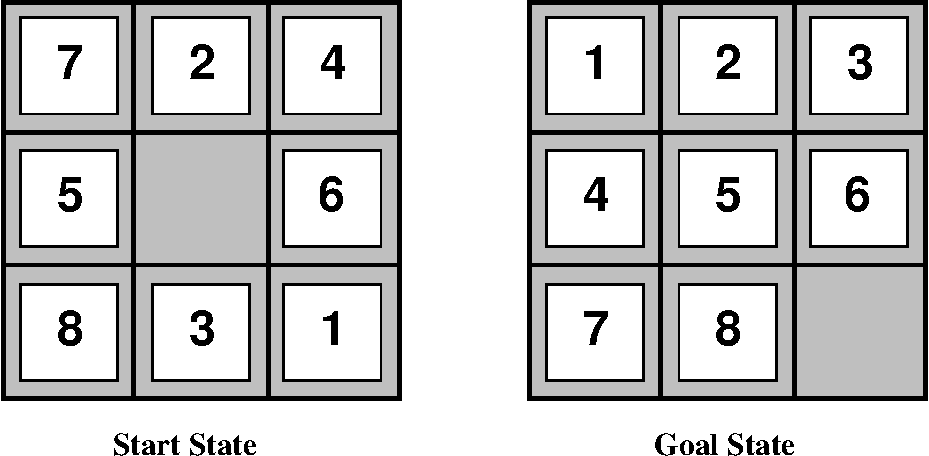
\includegraphics[height=1.25in]{8-puzzle.pdf}
	\end{center}
	\begin{tabular}{ll}
		\medskip
		\uncover<2->{\color{blue}Misplaced Tiles}    & \uncover<3->{\footnotesize $h(n) = 6$} \\
		\medskip
		\uncover<4->{\color{blue}Manhattan Distance} & \uncover<5->{\footnotesize $h(n) = 4 + 0 + 3 + 3 + 1 + 0 + 2 + 1$} \\
	\end{tabular}
\end{frame}
\begin{frame}{Heuristic Quality}
	\begin{block}{All heuristics were not created equal}
		\begin{tabular}{rrr}
			                      & \color{blue}Misplaced Tiles & \color{blue}Manhattan Distance \\
			\color{blue} 4 moves  &                    13 nodes &                       12 nodes \\
			\color{blue} 8 moves  &                    39 nodes &                       25 nodes \\
			\color{blue}12 moves  &                   227 nodes &                       73 nodes \\
			\color{blue}16 moves  &                  1301 nodes &                      211 nodes \\
			\color{blue}20 moves  &                  7276 nodes &                      676 nodes \\
		\end{tabular}
	\end{block}
\end{frame}
\begin{frame}{Heuristic Dominance}
	\begin{block}{Dominance}
		$h_1$ \textbf{dominates} $h_2$ if for all $n$, $h_1(n) \geq h_2(n)$
		\\ \bigskip
		Which one dominates?
		\begin{itemize}
			\item Misplaced Tiles
			\item<1-|alert@2-> Manhattan Distance
		\end{itemize}
	\end{block}
	\begin{block}<3->{Dominance = Efficiency}
		A* with $h_1$ will never expand more nodes than A* with $h_2$
		\\ \bigskip
		\alert{Why?} \uncover<4->{Every node with $h(n) < C^{*} - g(n)$ is expanded}
	\end{block}
\end{frame}

\subsection{Inventing Heuristics}
\begin{frame}{Relaxed Problems}
	\begin{block}{The 8-Puzzle}
		\begin{tabular}{ll}
			\bf Problem                                  & \bf Heuristic\\
			\hline
			\uncover<2->{Tiles move anywhere}            & \uncover<3->{Misplaced Tiles} \\
			\uncover<4->{Tiles move to adjacent squares} & \uncover<5->{Manhattan Distance} \\
		\end{tabular}
	\end{block}
	
	\begin{block}<6->{Generating heuristics}
		Exact solution to relaxed problem $\Rightarrow$ consistent heuristic
		\\ \bigskip
		\alert{Why?}
		\uncover<7->{
		\begin{itemize}
			\item Solution in original problem is also solution in relaxed
			\item Heuristic is exact cost in relaxed $\Rightarrow$ triangle inequality
		\end{itemize}
		}
	\end{block}
\end{frame}

\subsection{Heuristic Examples}
\begin{frame}{Traveling Salesman Problem}
	\begin{columns}
		\begin{column}{2in}
			\begin{block}{Problem}
				Visit all cities exactly once, minimum distance
			\end{block}
			\begin{center}
				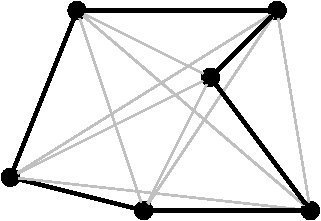
\includegraphics[width=2in]{tsp.pdf}
			\end{center}
		\end{column}
		\pause
		\begin{column}{2in}
			\begin{block}{Heuristic}
				Minimum spanning tree \\
				Solvable in $O(n^2)$
			\end{block}
			\begin{center}
				\visible<2>{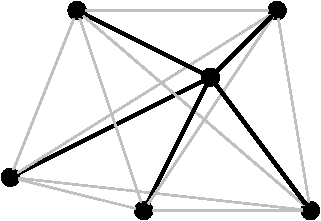
\includegraphics[width=2in]{mst.pdf}}%
			\end{center}
		\end{column}
	\end{columns}
\end{frame}
\begin{frame}{Bag Generation}
	\begin{block}{Determine the original order of a bag of words}
		\begin{description}
			\item[Initial] Full bag, empty sentence
			\item[Actions] Pop from bag, add to sentence
			\item[Goal] Empty bag, full sentence
			\item[Score] \small $P(w_1|\mbox{Start})P(w_2|w_1)P(w_3|w_2)\ldots P(x_n|x_{n-1})$
		\end{description}
	\end{block}
	\begin{center}
		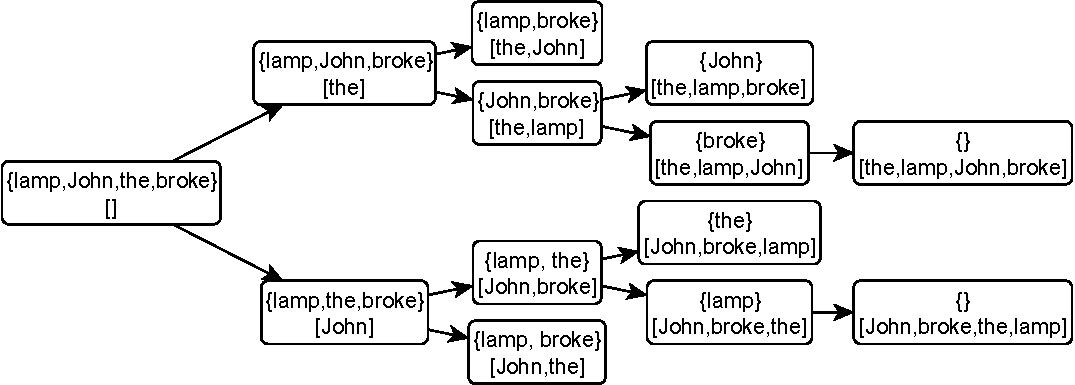
\includegraphics[width=4in]{bag-generation-search.pdf}
	\end{center}
\end{frame}
\begin{frame}{A Bag Generation Heuristic}
	\begin{columns}
		\begin{column}{2in}
			\begin{block}{Node}
				\texttt{$\{$lamp, the$\}$} \\
				\texttt{[John, broke]}
			\end{block}
			\begin{block}{Word Probability Estimates}
				\begin{tabular}{ll}
				the  & \uncover<2->{0.005} \\
				lamp & \uncover<3->{0.004} \\
				\end{tabular}
			\end{block}
			\begin{block}{h(n)}
				\uncover<4->{$0.005 * 0.004 = 0.00002$}
			\end{block}
		\end{column}
		\begin{column}{2in}
			\begin{tabular}{|ll|l|}
			\hline
			John  & the  & 0.0009 \\
			broke & the  & 0.005 \\
			the   & the  & 0.0 \\
			lamp  & the  & 0.0009 \\
			\hline
			\hline
			John  & lamp & 0.0 \\
			broke & lamp & 0.0 \\
			the   & lamp & 0.004 \\
			lamp  & lamp & 0.0 \\
			\hline
			\end{tabular}
		\end{column}
	\end{columns}
\end{frame}


\section{Local Search}
\begin{frame}{Local Search}
	\begin{block}{Sometimes only the goal matters (not the path)}
		\begin{itemize}
			\item 8-Queens
			\item Bag Generation
			\item Job Scheduling
		\end{itemize}
	\end{block}
	\begin{block}<2->{Iterative Improvement}
		Single \textit{current} state, explores neighbors
		\\ \medskip
		\begin{tabular}{ll}
			\uncover<3->{Memory?}   & \uncover<4->{$O(1)$} \\
			\uncover<5->{Optimal?}  & \uncover<6->{\textit{Usually not}} \\
			\uncover<7->{Complete?} & \uncover<8->{\textit{Usually not}} \\
		\end{tabular}
	\end{block}
\end{frame}
\begin{frame}{Example: Travelling Salesperson Problem}
	\begin{block}{Problem}
		Visit all cities exactly once, minimum distance
	\end{block}
	\begin{description}
		\item[Start] A random complete tour
		\item[Move] Swap a pair to reduce total distance
	\end{description}
	\begin{center}
		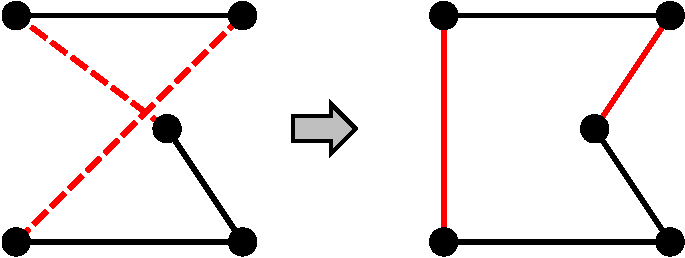
\includegraphics[height=1in]{tsp-sequence.pdf}
	\end{center}
	Achieves 1\% of optimal with thousands of cities
\end{frame}
\begin{frame}{Example: $n$-queens}
	\begin{block}{Problem}
		Put $n$ queens on an $n \times n$ board \\
		No two queens	on the same row, column, or diagonal
	\end{block}
	\begin{description}
		\item[Start] All queens placed randomly
		\item[Move] Move a queen to reduce conflicts
	\end{description}
	\begin{center}
		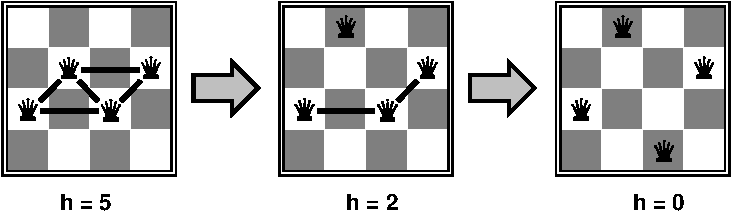
\includegraphics[height=1in]{4-queens-iterative.pdf}
	\end{center}
	Can solve $n$-queens problems for, e.g. $n = 1$ million
\end{frame}

\subsection{Hill Climbing}
\begin{frame}[fragile]{Hill Climbing}
	\scriptsize
	\begin{lstlisting}
		def hill_climb(problem):
		
		    # start at the problem's initial state
		    current = Node(problem.initial_state)
		    while True:
		
		        # select the neighboring state with the best score
		        state_scores = []
		        get_successors = problem.get_successors
		        for state, score in get_successors(current.state):
		            state_scores.append((score, state))
		        best_score, best_state = max(state_scores)
		
		        # if no neighbors are better, return the current
		        if best_score < current.score:
		            return current.state
		
		        # otherwise, move current to the best state
		        current = Node(best_state, best_score)
	\end{lstlisting}
\end{frame}
\begin{frame}{Hill Climbing}
	\begin{center}
		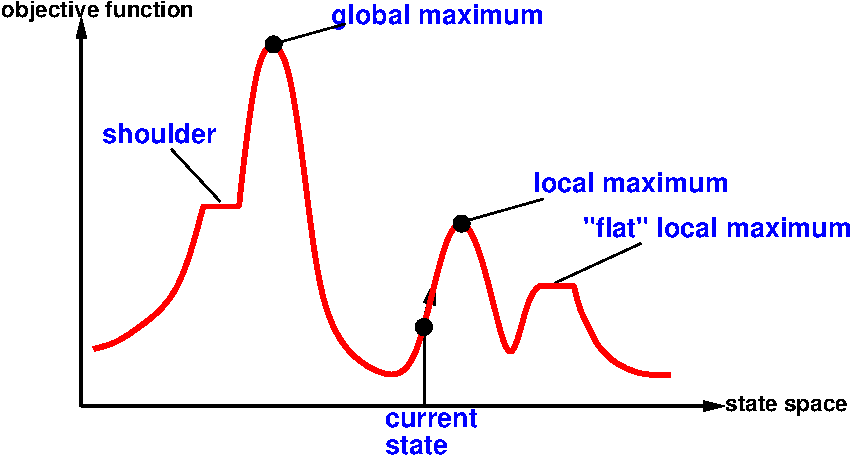
\includegraphics[width=4in]{hill-climbing.pdf}
	\end{center}
\end{frame}

\subsection{Random Hill Climbing}
\begin{frame}{Un-Sticking Hill Climbing}
	\begin{block}{Sideways Moves}
		Allow moving to neighbors as good as the current
	\end{block}
	\begin{block}<2->{Stochastic Hill Climbing}
		Choose randomly from \textit{all} neighbors that improve score
	\end{block}
	\begin{block}<3->{Random Restart Hill Climbing}
		Generate a new initial state and try again \uncover<4->{\alert<4->{Complete!}}
	\end{block}
	\begin{block}<5->{Simulated Annealing}
		Some bad moves; gradually decrease size and frequency \\
		\uncover<6->{\alert<6->{Complete and Optimal if ``gradual'' enough}}
	\end{block}
\end{frame}
\begin{frame}[fragile]{Simulated Annealing}
	\scriptsize
	\begin{lstlisting}
		def simulated_annealing(problem, get_temperature):
		    current = Node(problem.initial_state)
		    for time in itertools.count():
		        
		        # stop when the temperature reaches zero
		        temperature = get_temperature(time)
		        if not temperature:
		            return current
		        
		        # select a random neighbor
		        get_successors = problem.get_successors
		        successors = get_successors(current.state)
		        state, score = random.choice(successors)
		        
		        # always move to the neighbor always if it's
		        # better, and sometimes if it's worse
		        change = score - current.score
		        prob = math.exp(change / temperature)
		        if change > 0 or random.random() < prob:
		            current = Node(state, score)
	\end{lstlisting}
\end{frame}

\subsection{Local Beam Search}
\begin{frame}{Local Beam Search}
	\begin{block}{Idea}
		Keep $k$ states instead of just one
	\end{block}
	\begin{block}<2->{vs. $k$ Random Restarts}
		\uncover<3->{
		One state has good neigbors, others have bad neighbors
		\begin{description}
			\item[Local Beam Search] All searches share good neighbors
			\item[$k$ Random Restarts] Other searches use bad neighbors
		\end{description}
		}
	\end{block}
	\begin{block}<4->{Variants}
		\begin{itemize}
			\item<5-> Keep $k$ best states
			\item<6-> Keep $k$ random states, probabilities based on scores
		\end{itemize}
	\end{block}
\end{frame}
\begin{frame}[fragile]{Local Beam Search}
	\scriptsize
	\begin{lstlisting}
		def local_beam_search(problem, k):
		    current = [problem.generate_state() for _ in range(k)]
		    while True:
		        
		        # get all neighbors of the current states
		        state_scores = []
		        for node in current:
		            get_successors = problem.get_successors
		            for state, score in get_successors(node.state):
		                
		                # return the first goal state generated
		                if problem.is_goal(state):
		                    return state
		                state_scores.append((score, state))
		        
		        # select the k best states to consider next time
		        current = []
		        for score, state in heapq.nlargest(k, state_scores):
		            current.append(Node(state, score))
	\end{lstlisting}
\end{frame}
\begin{frame}{Genetic Algorithms}
	\begin{block}{Idea}
		\begin{itemize}
			\item Stochastic local beam search
			\item Successors generated from \textbf{pairs} of states
		\end{itemize}
	\end{block}
	\begin{center}
		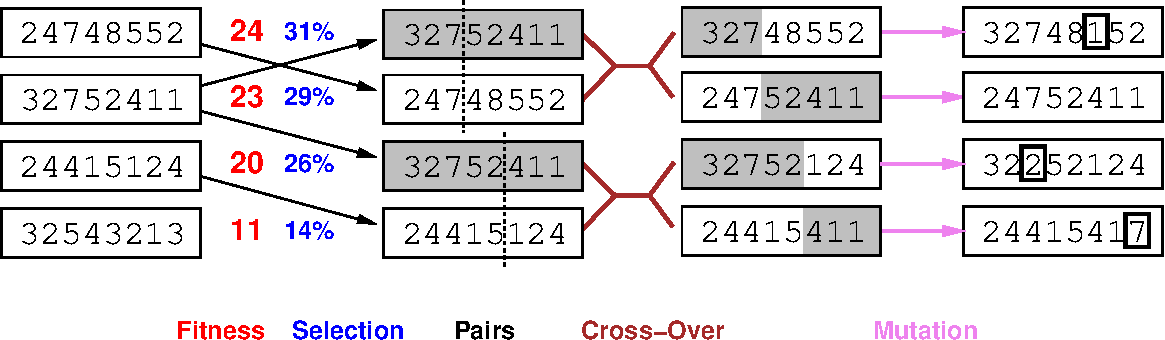
\includegraphics[width=4in]{genetic.pdf}
	\end{center}
\end{frame}
\begin{frame}{Genetic Algorithms}
	\begin{block}{Requirements}
		\begin{itemize}
			\item States must be encoded as strings
			\item Substrings must be meaningful components \\
			      \uncover<2->{\alert<2->{or crossover is pointless!}}
		\end{itemize}
	\end{block}
	\begin{center}
		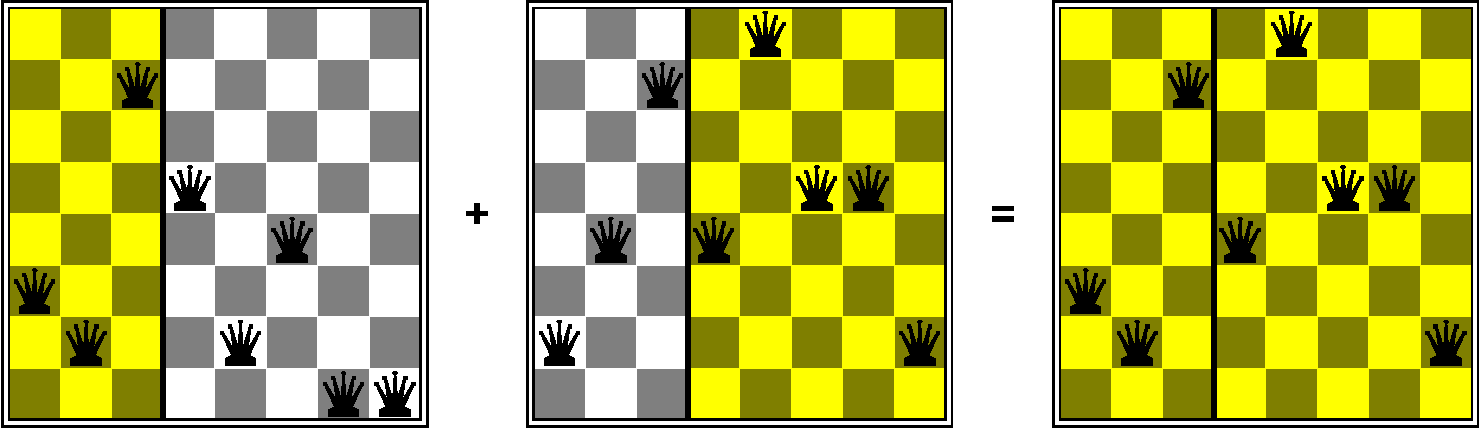
\includegraphics[width=4in]{8-queens-crossover.pdf}
	\end{center}
\end{frame}

\section{Advanced Search}

\subsection{Continuous Search Spaces}
\begin{frame}{Continuous Search Spaces}
	\begin{block}{Problem}
		Place 3 airports in Romania, minimizing
		$\sum\limits_{a \in \mbox{\textit{\scriptsize airports}}}
		 {\sum\limits_{c \in \mbox{\textit{\scriptsize cities}}}
		  {(x_c - x_a)^2 + (y_c - y_a)^2}}$
	\end{block}
	\begin{block}<2->{As a Search Problem?}
		\uncover<3->{
		But there are $\infty$ actions from each state!
		}
	\end{block}
	\begin{block}<4->{Solutions}
		\begin{description}
			\item[Discretize] each action moves $\pm\delta$ in $x$ or $y$ direction
			\item[Gradient] each action moves $\alpha\nabla f(x)$
		\end{description}
	\end{block}
\end{frame}

\subsection{Online Search}
\begin{frame}{Online Search}
	\begin{block}{Problem}
		Successor function is not available until a state is visited, \\
		e.g. robot exploration, maze problems
	\end{block}
	\begin{block}<2->{Solution: Learning Real-Time A*}
		Augment hill climbing with memory
		\begin{center}
			\only<-2>{\invisible{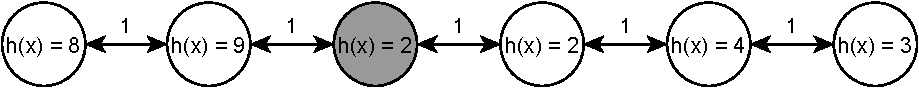
\includegraphics[width=4in]{lrta-star-1.pdf}}}%
			\only<3>{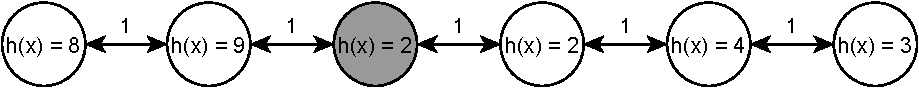
\includegraphics[width=4in]{lrta-star-1.pdf}}%
			\only<4>{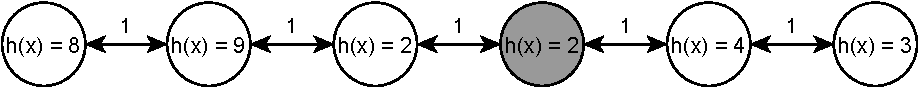
\includegraphics[width=4in]{lrta-star-2.pdf}}%
			\only<5>{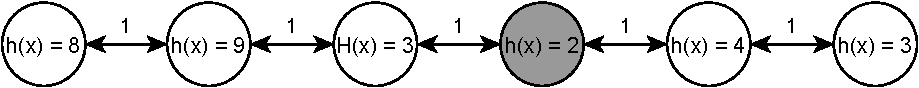
\includegraphics[width=4in]{lrta-star-3.pdf}}%
			\only<6>{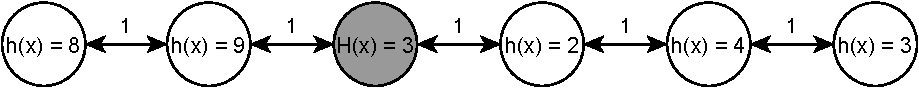
\includegraphics[width=4in]{lrta-star-4.pdf}}%
			\only<7>{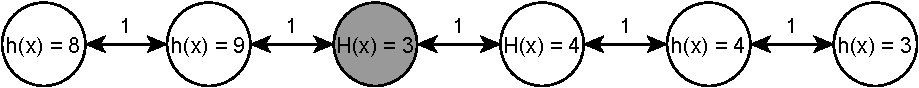
\includegraphics[width=4in]{lrta-star-5.pdf}}%
			\only<8>{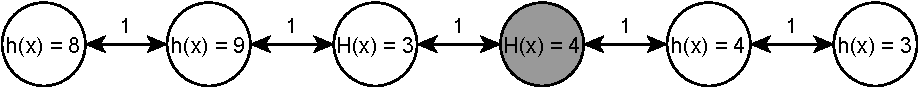
\includegraphics[width=4in]{lrta-star-6.pdf}}%
			\only<9>{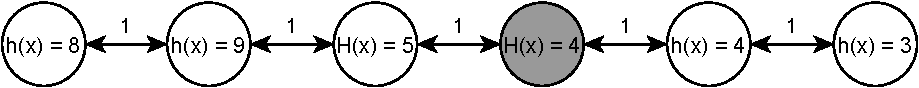
\includegraphics[width=4in]{lrta-star-7.pdf}}%
			\only<10->{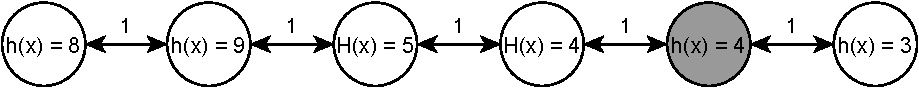
\includegraphics[width=4in]{lrta-star-8.pdf}}%
		\end{center}
		\uncover<11>{Complete in finite, safely explorable environments}
	\end{block}
\end{frame}

\part{Key Points}
\begin{frame}{Key Points}
	\begin{block}{Heuristics}
		\begin{itemize}
			\item Dominance
			\item Relaxed Problems
		\end{itemize}
	\end{block}
	\begin{block}{Search Algorithms}
		\begin{itemize}
			\item Best-First (Greedy) Search
			\item A* Search
			\item Hill Climbing
			\item Simulated Annealing
			\item Local Beam Search
			\item Discretized Search
			\item LRTA* Search
		\end{itemize}
	\end{block}
\end{frame}

\end{document}


